\documentclass{ltjsarticle}
\usepackage{luatexja}
\usepackage{graphicx}
\usepackage[top=2cm, bottom=2cm, left=1cm, right=1cm, includefoot]{geometry}

\title{実験レポート}
\author{HUIT はんちゃん}
\date{\today}

\begin{document}

\maketitle

\section*{目的}
オシロスコープの使い方を習得する。

\section*{方法}

オシロスコープを以下の手順で使用する。

\begin{enumerate}
    \item 電源を接続する\\ノイズ抑制、感電防止、測定対象やオシロスコープの故障防止のため、できるだけ接地の取れる電源を使用する。
    \item プローブの接続・設定\\全てのチャンネルで、プローブの倍率(1 倍、10 倍等)とオシロスコープの倍率の設定が一致している
          ことを確認する。変更できる場合、通常は 10 倍を使用する\footnote{10 倍では測定対象にプローブやオシロスコープが与える影響が小さくなり、測定精度が向上する。}。複数チャンネルを測定する場合、可能
          であればスキューの設定も行う\footnote{プローブの遅延分をオシロスコープ側で打ち消すことができる。}。
    \item プローブの調整・検査\\受動プローブでは、オシロスコープから出ている調整用の方形波出力を測定しながら、プローブとオシ
          ロスコープの接続部の調整部を調整用ドライバーで回し、整った方形波になるように調整する。このと
          き、GND も接続して行う\footnote{ プローブとオシロスコープの組み合わせを変えたときや、接続するチャンネルを変更したときは必ず行う。}。\\
          \begin{figure}[h]
              \centering
              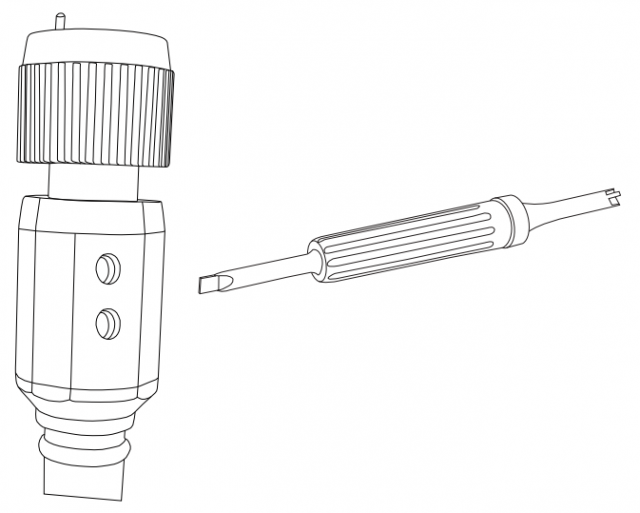
\includegraphics[height=5cm]{prove_calb.png}
              \caption{調整部と調整用ドライバー}
          \end{figure}
    \item 測定点との接続\\GND プローブを先に測定対象の GND に接続し、プローブの先端を出してテストピンなどに引っ掛
          ける\footnote{高周波測定の場合、GND と波形の測定を行い、まとめる。}。
    \item 電圧軸スケールとオフセットの調整\\画面の上下に波形がはみ出ないように、電圧軸のスケールとオフセットを調整する\footnote{波形が画面からはみ出る状態では、画面に表示されている部分も正しい波形になっていないことがある}。
    \item トリガーの設定\\通常は振幅の中央付近でトリガーがかかるようにする\footnote{波形が最も急峻に変化する部分が良い。}。
    \item 時間軸スケールの調整\\波形の 2 周期分など、波形の特徴が掴める時間軸に合わせる。
    \item 値の測定
          \begin{itemize}
              \item 周期は、振幅の中央付近のある電圧を上(もしくは下)に通過する時間の間隔をカーソルを使用し
                    て読み取る\footnotetext{もちろん某自然科学実験の動画のように正弦波のピークの間隔を測定してはいけない。}。
              \item 電圧は・・・
          \end{itemize}
    \item 波形を確認する。必要なら波形の画像を USB メモリーや LAN を通して PC に取り込む。

\end{enumerate}

\section*{測定}
別紙。

\section*{測定結果の評価}
方形波の測定ではオーバーシュートが観測された。実験者がプローブの調整をし忘れてしまった疑いが大き
い。また、波形の時間軸方向のスケールが大きすぎるため、立ち上がり、立下り部分の評価ができない。正弦
波の測定では、実験者が周期の測定時にピークの間隔を測定してしまったため、正確な周期がわからなくなっ
てしまった(画像の周期は画像からの推定であり、あまり正確ではない)。

\section*{感想}
昨日はバイト先でプローブの先端の部品を折ってしまった。幸いアロンアルファで修理することができた
が、先端だけで 10 万円するらしい。自然科学実験で使ったくらいのオシロスコープは本体数十万円、プロー
ブ 1,2 万円

\begin{figure}[p]
    \centering
    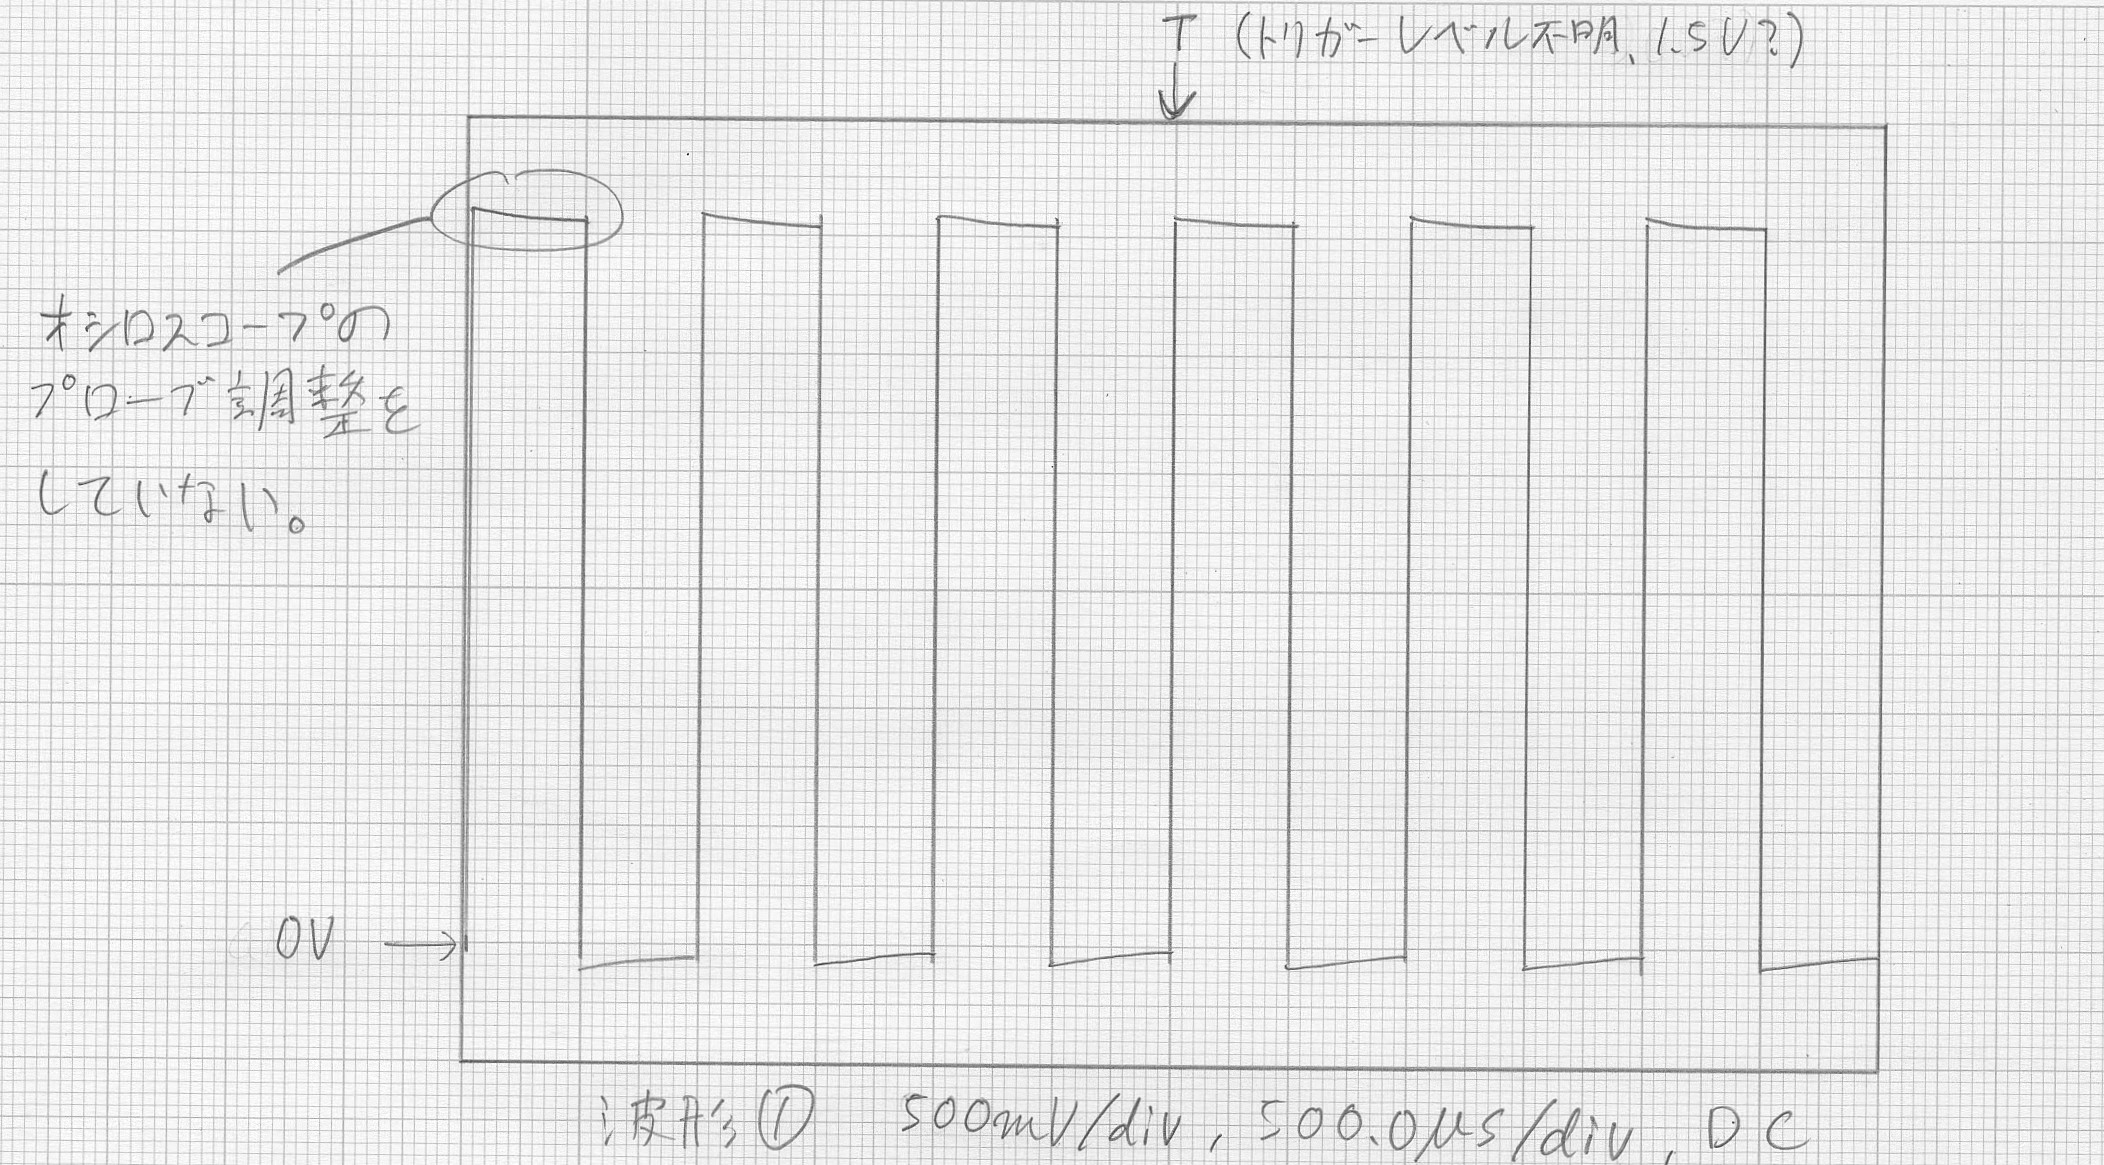
\includegraphics[height=8cm]{sq_wave.jpg}
    \caption{方形波の測定}
\end{figure}

\begin{figure}[p]
    \centering
    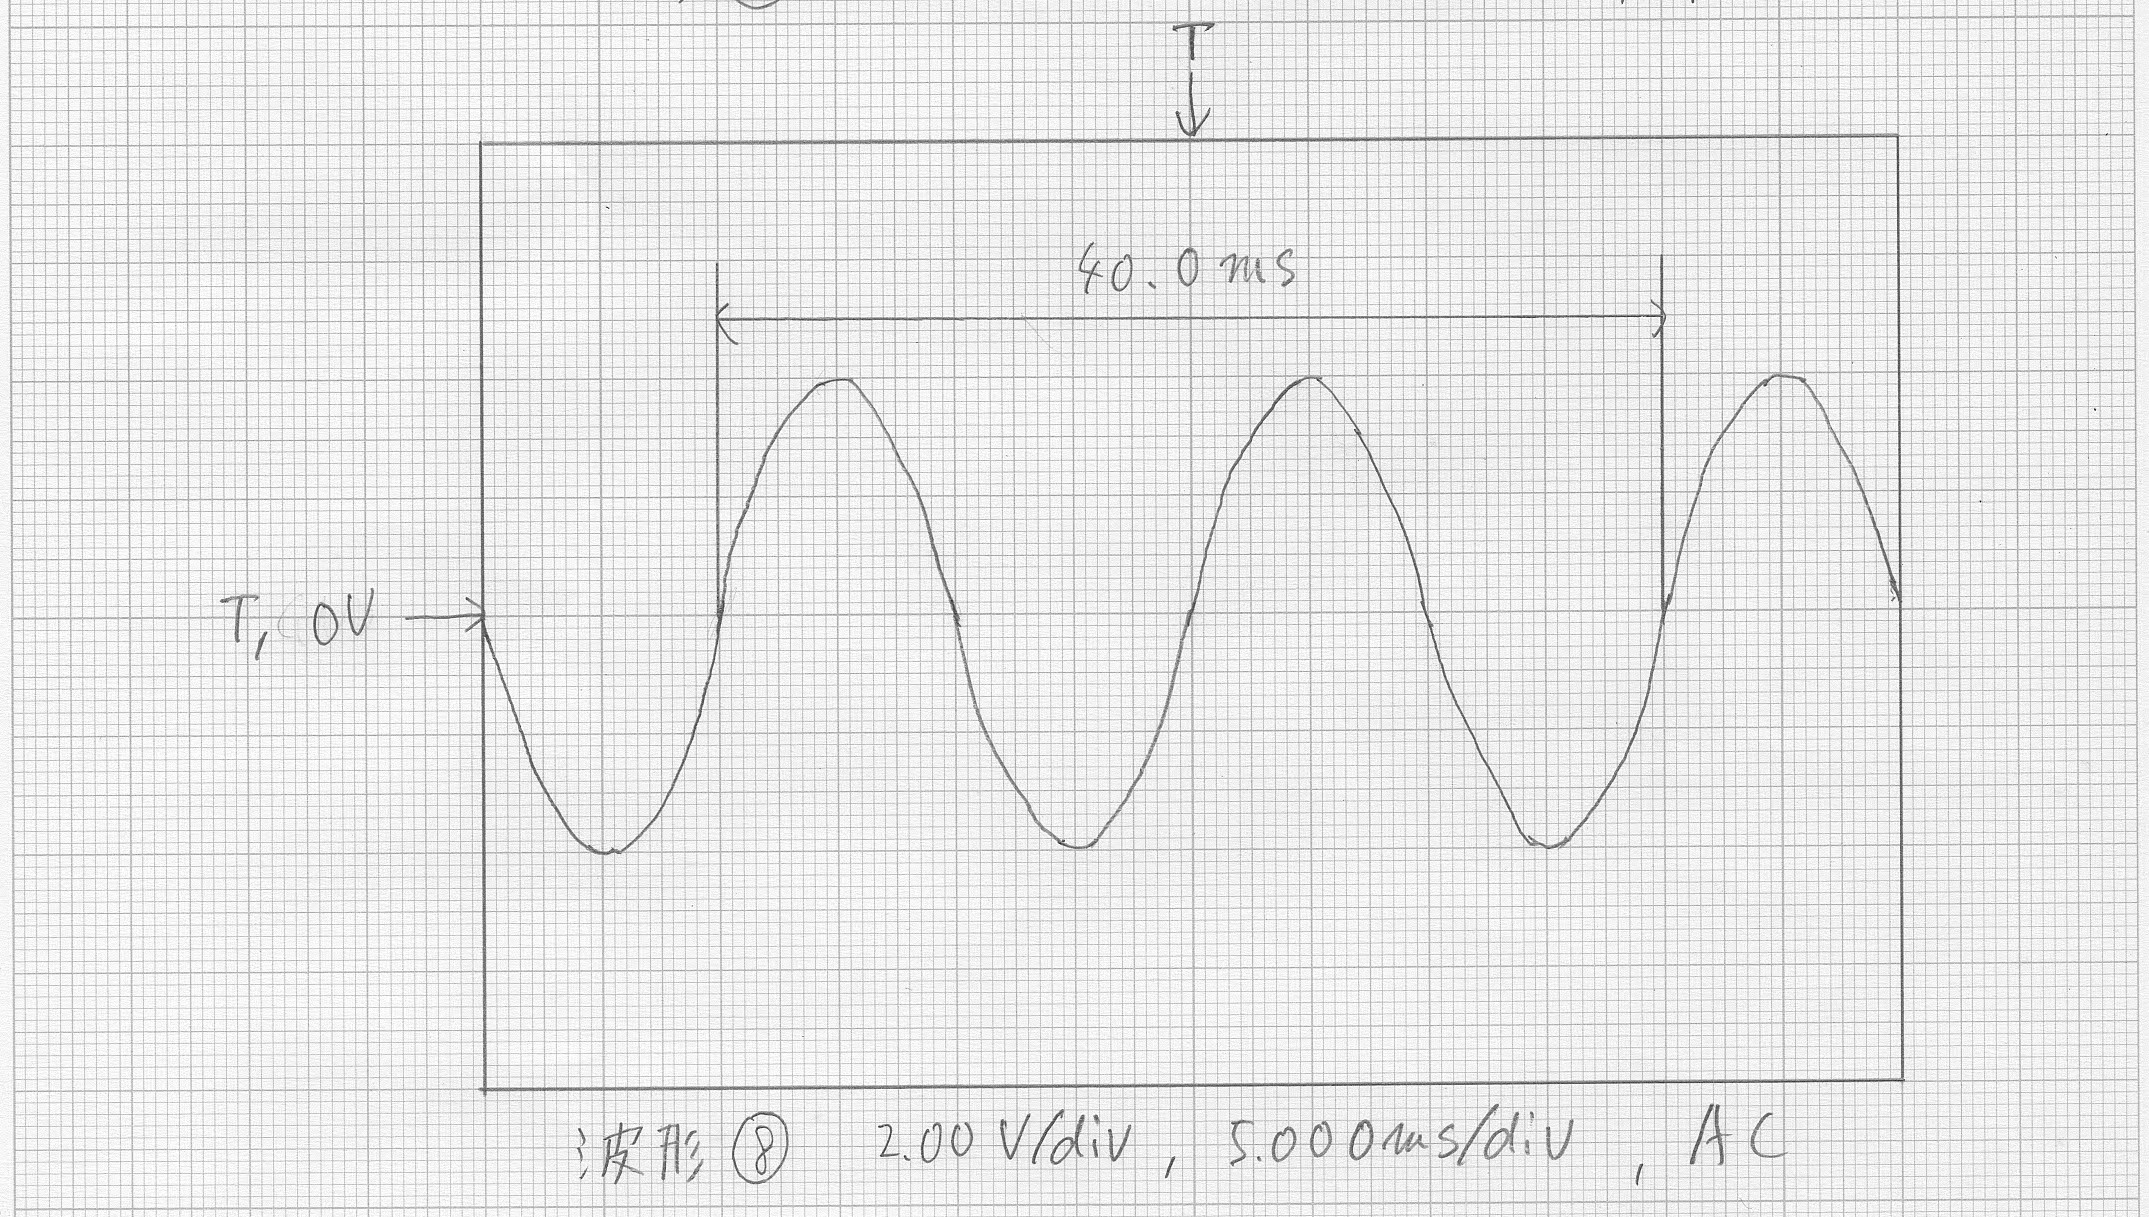
\includegraphics[height=8cm]{sine_wave.jpg}
    \caption{正弦波の測定}
\end{figure}

\end{document}